\documentclass{article}
\usepackage{graphicx}
\usepackage{amsmath}
\usepackage{subcaption}

\usepackage[final]{neurips_2023}

\usepackage[utf8]{inputenc} % allow utf-8 input
\usepackage[T1]{fontenc}    % use 8-bit T1 fonts
\usepackage{hyperref}       % hyperlinks
\usepackage{url}            % simple URL typesetting
\usepackage{booktabs}       % professional-quality tables
\usepackage{amsfonts}       % blackboard math symbols
\usepackage{nicefrac}       % compact symbols for 1/2, etc.
\usepackage{microtype}      % microtypography
\usepackage{xcolor}         % colors


\title{Classification problem on MNIST dataset}

\author{
  Antoni Kowalczuk
}

\begin{document}
\maketitle

\section{Introduction}
The classification task is about answering the following question: given a sample, determine which known categories/classes it belongs. Training a machine learning algorithm to be able to perform well on this task can be challenging since there is an infinite number of possible approaches, mainly in the space of the model selection, applied preprocessing of the training data, and the method of training the algorithm, i.e., adjusting the values of its parameters to have desired values to have high classification accuracy on the evaluation set.

In this assignment, I test multiple machine learning techniques to enhance the training and compare the results on an MNIST dataset (see \ref{subsec:mnist}). I also test the differences between the two machine learning algorithms. Results are then analyzed using $2^4$ factorial design. This assignment aims to show that the machine learning algorithm's choice and the training data preprocessing can significantly impact the algorithm's performance.

\section{Background}

\subsection{MNIST dataset}
\label{subsec:mnist}

\begin{figure}[ht]
    \centering
    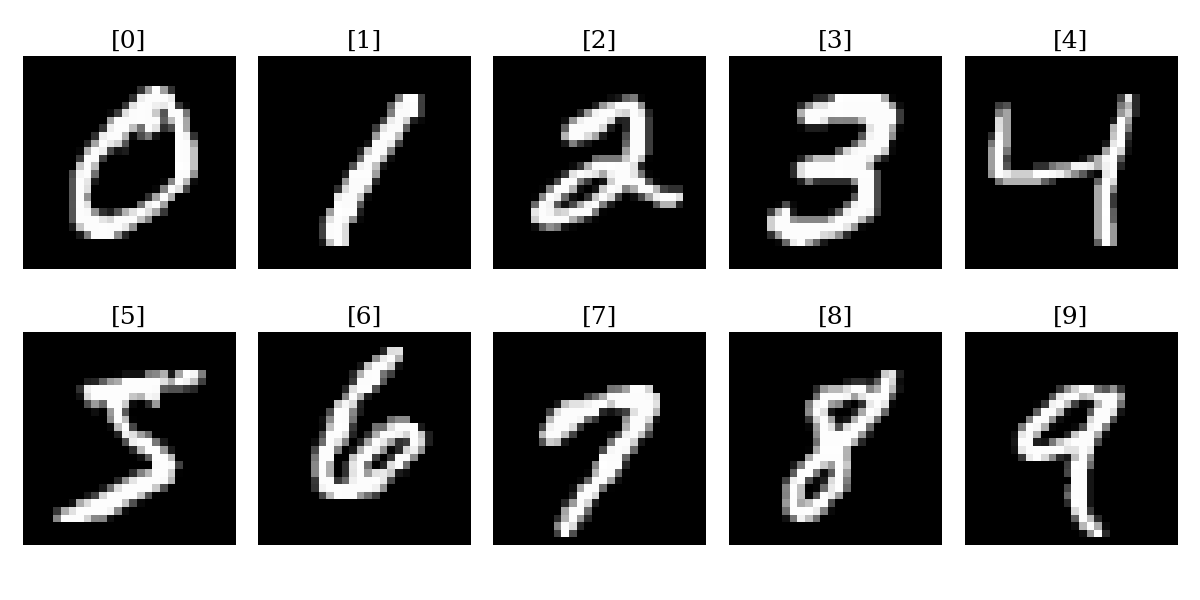
\includegraphics[width=\textwidth]{mnist.png}
    \caption{Sample from the MNIST dataset}
    \label{fig:mnist_sample}
\end{figure}

The MNIST dataset is a collection of 70,000 images of handwritten digits. Each image is a 28x28 pixel grayscale image. The dataset is widely used for training and testing machine learning algorithms, especially in computer vision. The dataset is available at \url{http://yann.lecun.com/exdb/mnist/}. The sample from the dataset is shown in Figure \ref{fig:mnist_sample}.

\subsection{Standard scaler}
\label{subsec:standard_scaler}
A standard scaler is a method of scaling the data to have zero mean and unit variance. It is a common preprocessing step in machine learning algorithms. It ensures that the data is not biased towards any particular feature. It also ensures that features with large values do not dominate the data. Data transformation is done by subtracting the mean and dividing it by the standard deviation. The formula for standard scaler is given by:
\begin{equation}
    x' = \frac{x - \mu}{\sigma}
\end{equation}
where $x$ is the original feature vector, $\mu$ is the mean of the feature vector and $\sigma$ is the standard deviation of the feature vector. Note that to avoid influencing our evaluation, we only fit the scaler (mean and the standard deviation) on the training data and then apply the same transformation to the test data.

\subsection{Principal component analysis}
\label{subsec:pca}
Principal component analysis (PCA) is a method of dimensionality reduction. It is used to reduce the number of features in the dataset. It is done by projecting the data onto a lower dimensional space. The new features are linear combinations of the original features. The new features are chosen in such a way that the variance of the data is maximized. The first principal component is the direction of the highest variance. The second principal component is the direction of the second highest variance, and so on. The formula for PCA is given by:
\begin{equation}
    X' = XW
\end{equation}
where $X$ is the original feature vector, $X'$ is the new feature vector, $W$ is the matrix of eigenvectors of the covariance matrix of $X$. Note that to avoid influencing our evaluation, we fit the PCA only on the training data and then apply the same transformation to the test data, as in the \ref{subsec:standard_scaler}.

\subsection{Data augmentation}
\label{subsec:augmentation}
Data augmentation is a method of increasing the size of the dataset by applying transformations to the original data. It is used to increase the size of the dataset when the original dataset is too small. It is also used to increase the robustness of the model. The transformations are chosen in such a way that they do not change the label of the data. In this assignment, I use the random vertical flip. It's a simple transformation that flips the image vertically. The transformation is applied with a probability of 0.5. The transformation is applied to the training data only. The effect of the transformation can be found in Figure \ref{fig:augmentation}.

\begin{figure}[ht]
    \centering
    \includegraphics[width=\textwidth]{vertical\_flip.png}
    \caption{Effect of the data augmentation}
    \label{fig:augmentation}
\end{figure}
Note that here we only aim to augment the training set. The evaluation set is left unchanged.

\subsection{Logistic regression}
\label{subsec:logistic_regression}
Logistic regression is a machine learning algorithm used for classification. It is a linear model that uses the logistic function to map the output to the probability of the class. The logistic function is given by:
\begin{equation}
    \sigma(x) = \frac{1}{1 + e^{-x}}
\end{equation}
The logistic regression model output is given by:
\begin{equation}
    \hat{y} = \sigma(\beta X)
\end{equation}
where $\hat{y}$ is the predicted label, $\beta$ is the weight vector and $X$ is the feature vector. The model is trained using gradient descent on the loss function, which is given by:
\begin{equation}
    L(\beta) = -\sum_{i=1}^{n} y_i \log(\hat{y_i}) + (1 - y_i) \log(1 - \hat{y_i})
\end{equation}
where $y_i$ is the true label and $\hat{y_i}$ is the predicted label.
The gradient:
\begin{equation}
    \nabla L(\beta) = X^T(\hat{y} - y)
\end{equation}
The weights are updated iteratively using the following formula:
\begin{equation}
    \beta = \beta - \alpha \nabla L(\beta)
\end{equation}
where $\alpha$ is the learning rate.

\subsection{Decision tree classifier}
\label{subsec:decision_tree}
The decision tree classifier is a machine learning algorithm used for classification. It is a non-linear model that uses a tree structure to map the output to the probability of the class. The tree structure is built by splitting the data into subsets based on the value of the feature. The splitting is done so that the subsets are as pure as possible. The purity of the subset is measured by the Gini impurity. The Gini impurity is given by:
\begin{equation}
    G = 1 - \sum_{i=1}^{n} p_i^2
\end{equation}
where $p_i$ is the probability of the class $i$ in the subset. The decision tree classifier model output is given by:
\begin{equation}
    \hat{y} = \arg\max_{i} p_i
\end{equation}
where $p_i$ is the probability of the class $i$ in the subset.

\section{\texorpdfstring{$2^k$} \text{ Factorial design}}
\label{sec:factorial_design}

\subsection{Effects estimation}
I use $2^4$ factorial design to analyse the results in this assignment. The factors tested are: applying scaling, decomposing the data to lower dimensions using PCA, applying data augmentation and different machine learning algorithms: logistic regression and decision tree classifier. The results are analyzed using the following formula:
\begin{equation}
    y = \beta_0 + \sum_{i=1}^{k} \beta_i x_i + \sum_{i=1}^{k} \sum_{j=i+1}^{k} \beta_{ij} x_i x_j + \sum_{i=1}^{k} \sum_{j=i+1}^{k} \sum_{l=j+1}^{k} \beta_{ijl} x_i x_j x_l + \beta_{1234} x_1 x_2 x_3 x_4
\end{equation}
where $y$ is the accuracy, our response variable, $x_i$ is the factor $i$ and $\beta_i$ is the coefficient of the factor $i$. The factors are $1$ (at high value) or $-1$ (at low value). The factor $x_{ij}$ denotes the interaction between the factor $i$ and the factor $j$ and $\beta_{ij}$ the coefficient of the factor $X_{ij}$. The factor $\beta_{1234}$ denotes the interaction between all the factors.

The covariates create a $2^4\times2^4$ matrix, denoted $\mathbf{X}$, with a first column of ones. The response variable vector is denoted by $\mathbf{Y}$, and the vector of coefficients by $\beta$ (the first element being an intercept). We don't know the values of the coefficients; therefore, we need to obtain the estimated values of the coefficients. The formula for it is as follows:
\begin{equation}
    \hat{\beta} = (\mathbf{X}^T \mathbf{X})^{-1} \mathbf{X}^T \mathbf{Y}
\end{equation}
Since the columns of the design matrix are orthogonal, we can simplify:
\begin{align}
    \mathbf{X^TX} = n\mathbf{I}                              \\
    \left(\mathbf{X^TX} \right)^{-1} = \frac{1}{n}\mathbf{I} \\
    \hat{\beta} = \frac{1}{n}\mathbf{X^TY}
\end{align}
Where $n=2^4$ is the number of observations. The estimated effect of the factor $i$ is given by:
\begin{equation}
    \widehat{Effect_i} = 2\hat{\beta_i}
\end{equation}

\subsection{Estimation of the standard deviation}
\label{subsec:std_estim}

Because in the test, I don't use replicates of the factor combinations, I can't use the estimator from the multiple linear regression because in MLR:
\begin{align}
    \mathbf{SSE} = \sum_{i=1}^{n} \left(y_i - \hat{y_i} \right)^2 \\
    \hat{\sigma}^2 = \frac{\mathbf{SSE}}{n-p}
\end{align}
and in this case $n=p$, so the denominator is zero. Therefore I use Method 1 from the course. It's based on the assumption that for $m$ higher order $j$, the effect of the $j$-th order interaction is negligible. For these $j$-s we have:
\begin{equation}
    \widehat{Effect_j} \sim N(0, \sigma_{effect}^2)
\end{equation}
We can then estimate the standard deviation of the effects by:
\begin{equation}
    \widehat{\sigma_{effect}} = \sqrt{\frac{1}{m} \sum_{j=n-m}^{n} \widehat{Effect_j}^2}
\end{equation}
$m$ is the number of higher-order interactions we assume to be negligible, and $n$ is the number of factors (including interactions).

\subsection{Hypothesis testing}
\label{subsec:hypothesis_testing}

The null hypothesis is that the factor does not affect the accuracy. The alternative hypothesis is that the factor affects the accuracy. The test statistic is given by:
\begin{equation}
    T_j = \frac{\widehat{Effect_j}}{\widehat{\sigma_{effect}}}
\end{equation}
Because we use the Method 1 (see Section \ref{subsec:std_estim}) of inferring the estimated standard deviation we have:
\begin{equation}
    T_j \sim t_{m}
\end{equation}
$m$ is the number of higher-order interactions we assume to be negligible, and $t_{m}$ is the Student's t-distribution with $m$ degrees of freedom.

At a significance level $\alpha$, the null hypothesis is rejected if:
\begin{equation}
    |T_j| \geq t_{\frac{\alpha}{2}, m}
\end{equation}

\section{Experimental setup}

\subsection{Dataset}
\label{subsec:dataset}
To evaluate the performance of a machine learning algorithm, a common approach is to divide the whole dataset into two parts: training set and evaluation set. The algorithm only "sees" the training set samples during training. Then, after the training procedure is finished, it is evaluated on the evaluation set, and the performance value is reported. This approach is used in this assignment.

I split the whole MNIST (see \ref{subsec:mnist}) dataset into 60k random training samples and 10k random evaluation samples. It's done once, and then I train algorithms in different setups on the training set. The same training set is used in all configurations of the factors to rule out the possible influence of a random split of the dataset on the results, which can be the case if I randomly split the dataset for each configuration of the factors.

The evaluation is then done on the evaluation set; similarly, as above, the evaluation set is the same for all configurations of the factors.

\subsection{Factors}
To test a generic approach a machine learning practitioner usually takes when faced with the classification task, I introduce the following factors to the experiment:
\begin{enumerate}
    \item \textbf{Factor A: Scaling} - scaling the data to have zero mean and unit variance (see \ref{subsec:standard_scaler}). The high value of this factor means that the data is scaled, low that it isn't. It has been shown that scaling the data can improve the machine learning algorithm's performance since the algorithm can converge faster. However, it is not always the case. Since the pixel values of the MINST dataset are contained between 0 and 255, scaling the data shouldn't significantly impact the algorithm's performance.
    \item \textbf{Factor B: PCA} - decomposing the data to lower dimension using PCA (see \ref{subsec:pca}). The high value of this factor means that the data is decomposed, low that it isn't. By applying this transformation, we lose some information, but we then focus on saving as important information as possible in the new vector space. This approach can improve the machine learning algorithm's performance in terms of overfitting. In this experiment, we downsize the feature space from $28\times28=784$ to $10$ dimensions.
    \item \textbf{Factor C: Augmentation} - applying data augmentation (see \ref{subsec:augmentation}), i.e., adding new samples to the training set using a random subset from the training set on which we apply the augmentation operation. The high value of this factor means that the training data is augmented, low that it isn't. It's a commonly used technique to generate more samples for the model to learn from without destroying the information contained in the data. More data to learn from is almost always beneficial for the machine learning algorithm's performance. In this experiment, I sample a random subset of $50\%$ of the training set and then perform a flipping operation. Note that not to introduce a new variable to the setup, the random subset is always the same for each configuration of the factors. If it isn't the case, it's necessary to introduce a new factor to the experiment since the differences between random subsets can influence the results.
    \item \textbf{Factor D: Algorithm} - choosing the machine learning algorithm. The high value of this factor means that the logistic regression algorithm (see \ref{subsec:logistic_regression}) is used, and low that the decision tree classifier (see \ref{subsec:decision_tree}) is used. Decision tree classifiers usually have greater learning capacity than logistic regression, effectively performing better on more complex tasks. However, they are more prone to overfitting, which can be problematic when the training data is small.
\end{enumerate}

The factors will stay at their levels since the implementation of the experiment in the software (see \ref{subsec:software_implementation}) assures it to be correct.

\subsection{Response}
A typical performance metric when it comes to the classification problem is accuracy, which is calculated as follows:
\begin{equation}
    \text{accuracy} = 100\%\times\frac{\text{number of correctly classified samples}}{\text{total number of samples}}
\end{equation}
Although we must be extra careful when using this metric, it can be misleading. For example, suppose we have a dataset with 90\% of samples belonging to class A and 10\% belonging to class B. In that case, a classifier that always predicts class A will have 90\% accuracy, which is a high value, but the classifier is useless. Such a dataset is often called "imbalanced" since the balance of the classes is skewed towards one (or more if dealing with a multiclass classification task) of them. Fortunately, the MNIST dataset is balanced, i.e., the number of samples belonging to each class is similar. Therefore I use accuracy as the response metric. It's continuous since it's a percentage value and bounded between 0 and 100\%, so it fits the factorial design.

During preparation for this experiment, I also considered other metrics, such as precision, recall, and F1 score. Still, they are not used in this assignment since precision and recall are useful when we care more about one class than the other, and the F1 score is a combination of precision and recall, so it's not needed to be used in this assignment.

The response is measured on the evaluation set (see \ref{subsec:dataset}). These measurements will be accurate since a software implementation (see \ref{subsec:software_implementation}) of the experiment does them.

\subsection{Design}
The design of the experiment is a full factorial design (see \ref{sec:factorial_design}) since all factors are at their levels. The number of runs is $2^4=16$ since we have $4$ factors, each with $2$ levels. Blocking is not used; all experiments are run in a single Python script (see \ref{subsec:software_implementation}). Replicates might be desirable to mitigate the influence of the randomness of the dataset split. They can be done by running the same set of combinations with multiple random splits of the dataset (see \ref{subsec:dataset}), but it's not done in this assignment. Randomization is not used since the order of the experiments doesn't matter.

I follow the approach described in \ref{subsec:std_estim} regarding the standard deviation estimation for the factors' effects estimates. $m$, in this case, is selected to contain all interactions of three or more factors, in this case, $m=5$.

\subsection{Software implementation}
\label{subsec:software_implementation}

The software implementation of the experiment is done in Python 3.10 using classic machine learning libraries: scikit-learn (algorithms), numpy and pandas (data manipulation), and scipy (statistics). The code is available in the \url{https://github.com/Ankowa/TMA4267_task_3/blob/main/run_all_experiments.py}. For Figure \ref{fig:factors_effect}, I use the matplotlib library. The calculation of the estimated standard deviation (see \ref{subsec:statistical_significance}) is done using interactive Jupyter Notebook, and the code used to generate Figure \ref{subsec:std_estim} is also there. Notebook is available in the \url{https://github.com/Ankowa/TMA4267_task_3/blob/main/prd.ipynb}.

\section{Results}

The final results are in Table \ref{tab:design_matrix}, and the factors estimated effects are in Figure \ref{fig:factors_effect}. Figure \ref{fig:effects_plots} shows the main effect and interaction plots.

\begin{table}[!ht]
    \centering
    \resizebox{\textwidth}{!}{
        \begin{tabular}{|r|r|r|r|r|r|r|r|r|r|r|r|r|r|r|r|r|r|}
            \textbf{} & \textbf{intercept} & \textbf{A} & \textbf{B} & \textbf{C} & \textbf{D} & \textbf{AB} & \textbf{AC} & \textbf{AD} & \textbf{BC} & \textbf{BD} & \textbf{CD} & \textbf{ABC} & \textbf{ABD} & \textbf{ACD} & \textbf{BCD} & \textbf{ABCD} & \textbf{Y} \\ \hline
            0         & 1                  & 1          & 1          & 1          & 1          & 1           & 1           & 1           & 1           & 1           & 1           & 1            & 1            & 1            & 1            & 1             & 72.38      \\
            1         & 1                  & 1          & 1          & 1          & -1         & 1           & 1           & -1          & 1           & -1          & -1          & 1            & -1           & -1           & -1           & -1            & 77.56      \\
            2         & 1                  & 1          & 1          & -1         & 1          & 1           & -1          & 1           & -1          & 1           & -1          & -1           & 1            & -1           & -1           & -1            & 77.65      \\
            3         & 1                  & 1          & 1          & -1         & -1         & 1           & -1          & -1          & -1          & -1          & 1           & -1           & -1           & 1            & 1            & 1             & 82.16      \\
            4         & 1                  & 1          & -1         & 1          & 1          & -1          & 1           & 1           & -1          & -1          & 1           & -1           & -1           & 1            & -1           & -1            & 85.39      \\
            5         & 1                  & 1          & -1         & 1          & -1         & -1          & 1           & -1          & -1          & 1           & -1          & -1           & 1            & -1           & 1            & 1             & 86.98      \\
            6         & 1                  & 1          & -1         & -1         & 1          & -1          & -1          & 1           & 1           & -1          & -1          & 1            & -1           & -1           & 1            & 1             & 89.49      \\
            7         & 1                  & 1          & -1         & -1         & -1         & -1          & -1          & -1          & 1           & 1           & 1           & 1            & 1            & 1            & -1           & -1            & 87.46      \\
            8         & 1                  & -1         & 1          & 1          & 1          & -1          & -1          & -1          & 1           & 1           & 1           & -1           & -1           & -1           & 1            & -1            & 74.34      \\
            9         & 1                  & -1         & 1          & 1          & -1         & -1          & -1          & 1           & 1           & -1          & -1          & -1           & 1            & 1            & -1           & 1             & 79.97      \\
            10        & 1                  & -1         & 1          & -1         & 1          & -1          & 1           & -1          & -1          & 1           & -1          & 1            & -1           & 1            & -1           & 1             & 77.87      \\
            11        & 1                  & -1         & 1          & -1         & -1         & -1          & 1           & 1           & -1          & -1          & 1           & 1            & 1            & -1           & 1            & -1            & 82.73      \\
            12        & 1                  & -1         & -1         & 1          & 1          & 1           & -1          & -1          & -1          & -1          & 1           & 1            & 1            & -1           & -1           & 1             & 79.32      \\
            13        & 1                  & -1         & -1         & 1          & -1         & 1           & -1          & 1           & -1          & 1           & -1          & 1            & -1           & 1            & 1            & -1            & 84.36      \\
            14        & 1                  & -1         & -1         & -1         & 1          & 1           & 1           & -1          & 1           & -1          & -1          & -1           & 1            & 1            & 1            & -1            & 83.98      \\
            15        & 1                  & -1         & -1         & -1         & -1         & 1           & 1           & 1           & 1           & 1           & 1           & -1           & -1           & -1           & -1           & 1             & 87.49      \\
        \end{tabular}
    }
    \caption{Design matrix}
    \label{tab:design_matrix}
\end{table}

\begin{figure}[!ht]
    \centering
    \includegraphics[width=\textwidth]{factors\_effect.png}
    \caption{The estimated effects of factors. The x-axis corresponding to the effect value is logarithmic. The green bar means statistically significant, red bar means not statistically significant.}
    \label{fig:factors_effect}
\end{figure}

\begin{figure}[!ht]
    \begin{subfigure}{0.49\textwidth}
        \centering
        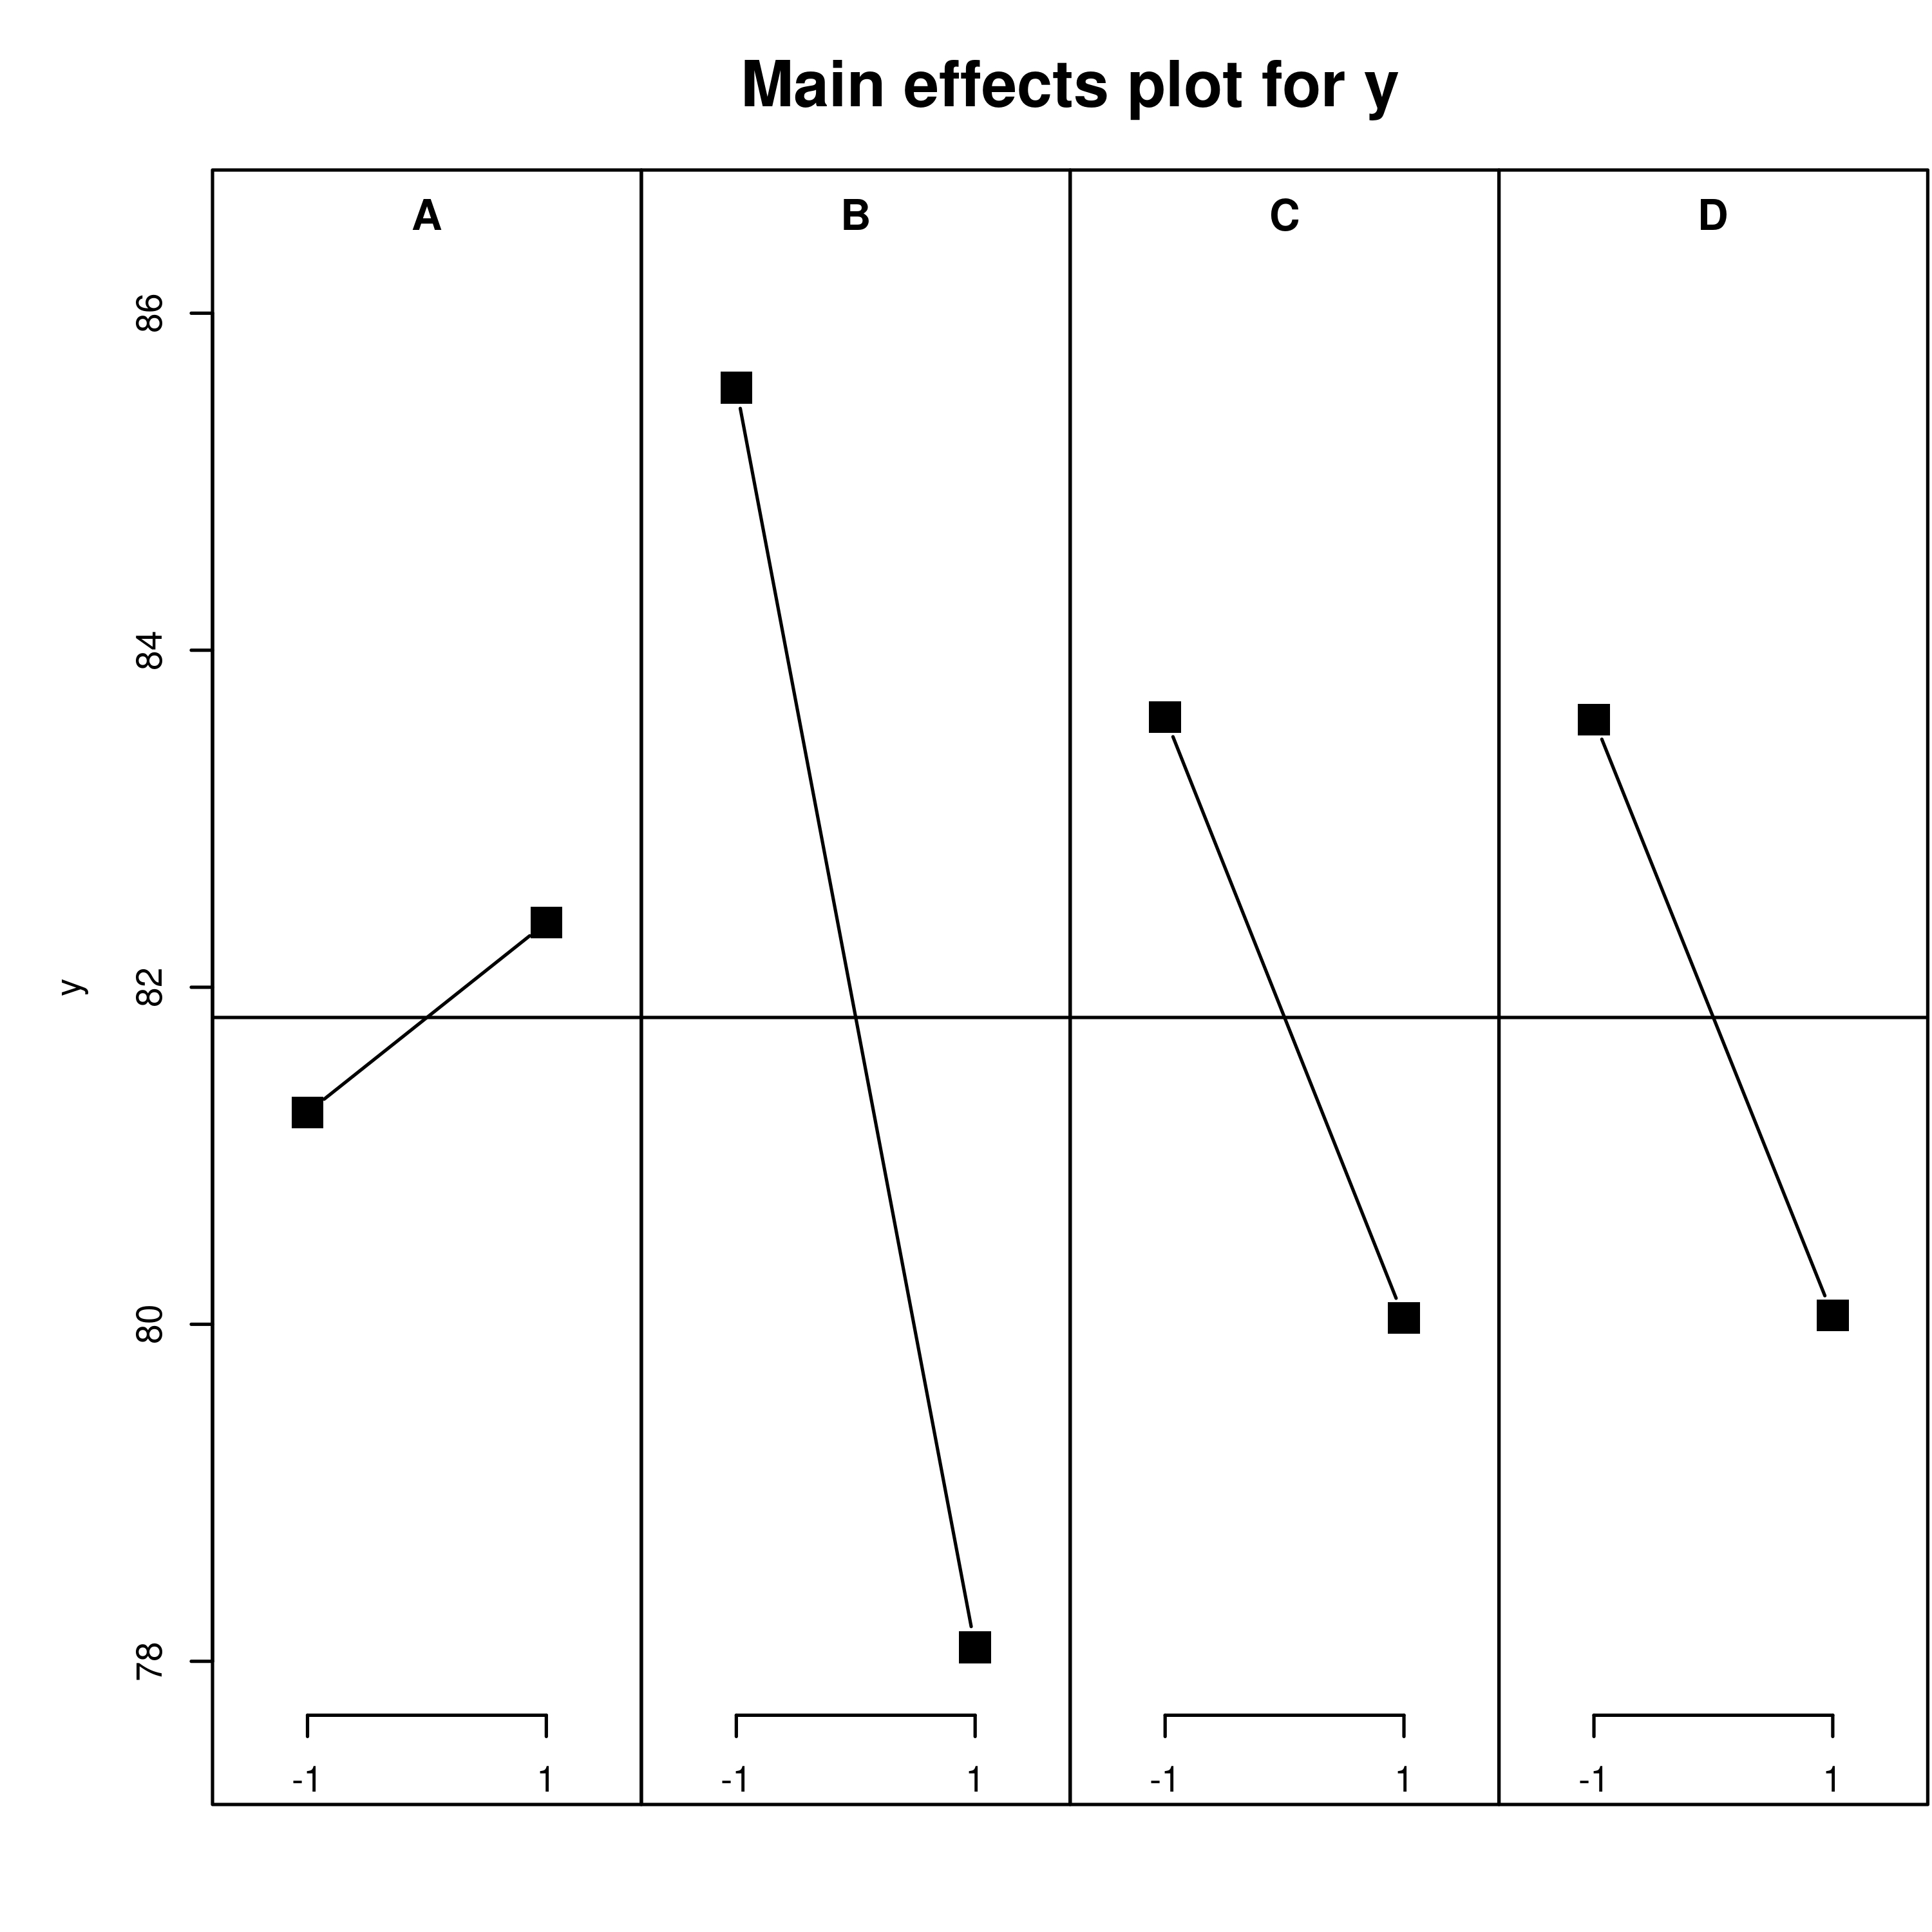
\includegraphics[width=\textwidth]{main_effects_plot.jpeg}
        \caption{Main effects plot}
        \label{fig:main_effects_plot}
    \end{subfigure}
    \begin{subfigure}{0.49\textwidth}
        \centering
        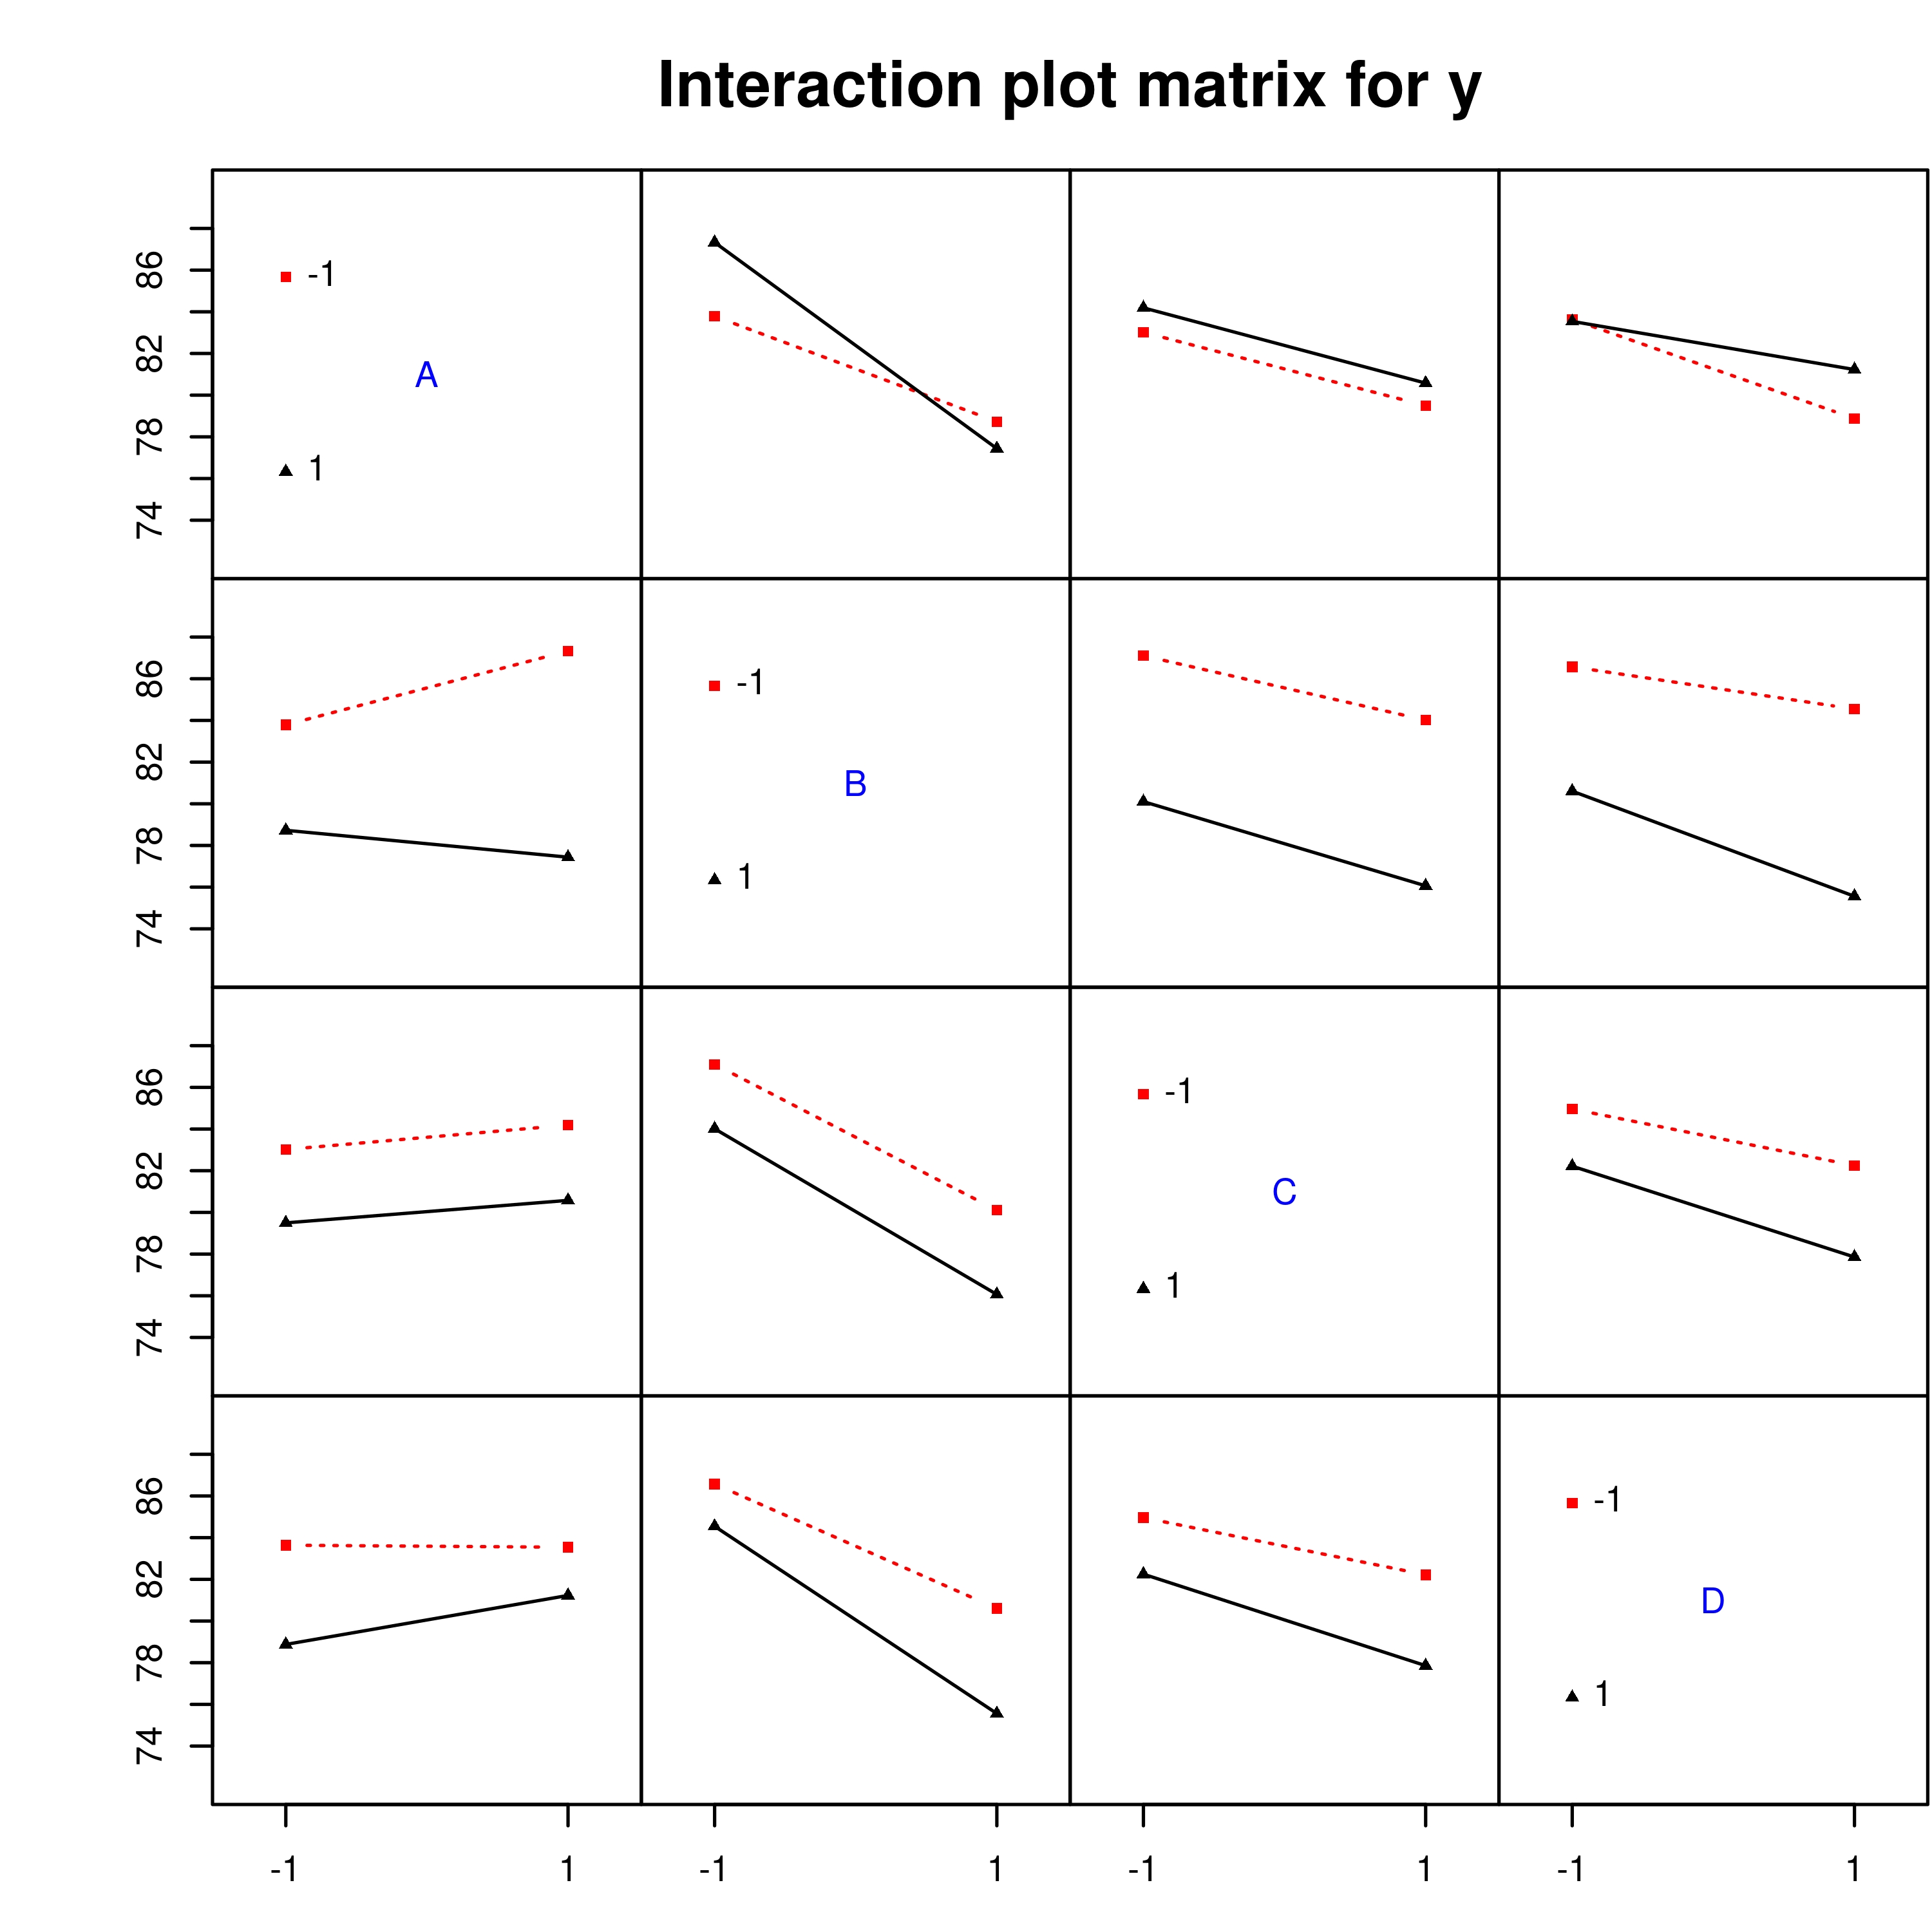
\includegraphics[width=\textwidth]{interaction_effects_plot.jpeg}
        \caption{Interaction effects plot}
        \label{fig:interaction_effects_plot}
    \end{subfigure}
    \caption{Effects plots}
    \label{fig:effects_plots}
\end{figure}

\subsection{Statistical significance}
\label{subsec:statistical_significance}

Following \ref{subsec:std_estim} we have:
\begin{gather}
    \widehat{\sigma_{effect}} = \sqrt{\frac{1}{5} \sum_{j=11}^{16} \widehat{Effect_j}^2} \\
    \widehat{\sigma_{effect}} = \sqrt{\frac{1}{5}\times\left[
            \left(-0.84875\right)^2
            + \left(-1.02375\right)^2
            + \left(-0.24875\right)^2
            + \left(0.46375\right)^2
            + \left(0.27375\right)^2
            \right]}                                                                             \\
    \widehat{\sigma_{effect}} = 0.65
\end{gather}
Following \ref{subsec:hypothesis_testing}, for a confidence level of $\alpha=95\%$ we have:
\begin{equation}
    t_{0.975, 5} = 2.571
\end{equation}
We test against the $H_0$ hypothesis for each factor $i$:
\begin{equation}
    \left| \frac{\widehat{Effect_i}}{\widehat{\sigma_{effect}}} \right| \geq t_{0.975, 5}
\end{equation}
Results are shown in Figure \ref{fig:factors_effect}.

\section{Analysis}

\subsection{Residual Plots}
The linear regression model fitted on the data from the experiments is almost perfectly accurate, with the highest residual of value $1.4\times10^{-14}$, which is negligible. Because of that, the residual plot is not very informative, therefore, not included in the assignment.

\subsection{Main effects}

\begin{itemize}
    \item Factor A: we can see that scaling the training data has little effect on the model performance. This is probably because the model is not very sensitive to the scale of the data, and the data is already well-scaled. Scaling is profitable in extreme cases, like one variable having orders of magnitude bigger variance than the other.
    \item Factor B: we can see that decomposing the data with PCA has a huge negative impact on the performance. Most likely, we are losing too much information in the process.
    \item Factor C: surprisingly, we observe a negative effect of augmenting the training data. Probably it's because flipping the data is not a good augmentation for this dataset, e.g., flipping the hand-written digit 5 will result in a 2, which is a completely different digit.
    \item Factor D: we see that the decision tree classifier performs way better than logistic regression.
\end{itemize}

\subsection{Interaction effects}

Even though none of the interactions are statistically significant, I point out the following observations:

\begin{itemize}
    \item Factor A and B: interestingly, when data is scaled, the negative effect of decomposing it into lower dimensions is amplified.
    \item Factor A and D: scaling doesn't matter when using a decision tree classifier. Given how this algorithm divides the hyperspace into regions, it's unsurprising since the divisions should be the same, just shifted. Intuitively, it benefits the logistic regression because it's a gradient-based algorithm, and the gradient is affected by the scale of the data.
    \item Factor C: augmenting is always bad, regardless of configuration. We should avoid it in this case.
    \item Factor B and D: PCA affects logistic regression more than decision tree classifier. This is probably because the decision tree classifier can extract more information from the data since it's more complex.
\end{itemize}

\subsection{Conclusion}

The best configuration is the one with the lowest error, which is the one with the following factors:

\begin{itemize}
    \item A: no scaling
    \item B: no PCA
    \item C: no augmentation
    \item D: decision tree classifier
\end{itemize}

\end{document}